\subsection{Das Restglied nach Lagrange}
In diesem Abschnitt werden mit dem Mittelwertsatz eine Formel für das $n$-te Restglied $R_n (x)=f(x)-T_n (x)$ der Taylorentwicklung herleiten. Damit werden wir beweisen können, dass einige der bereits hergeleiteten Taylorreihen tatsächlich gegen die ursprüngliche Funktion konvergieren. Ausserdem können wir mit dieser Formel den Fehler abschätzen, den man macht, wenn man einen Funktionswert durch den Wert des Taylorpolynoms $n$-ten Grades approximieren.

\textbf{Das Restglied $R_0(x)$}

Sei \( f \) eine differenzierbare Funktion und sei \( T_{0,x_0}(x) \) deren Taylorpolynom nullten Grades mit Entwicklungsstelle \( x_0 \), das heisst:
\[ T_{0,x_0}(x) = f(x_0) \]

Das Restglied \( R_0(x) \) ist dann die Differenz zwischen der Funktion \( f \) und der Taylorentwicklung \( T_{0,x_0}(x) \):
\[ R_0(x) = f(x) - T_{0,x_0}(x) = f(x) - f(x_0)\]
\begin{center}
	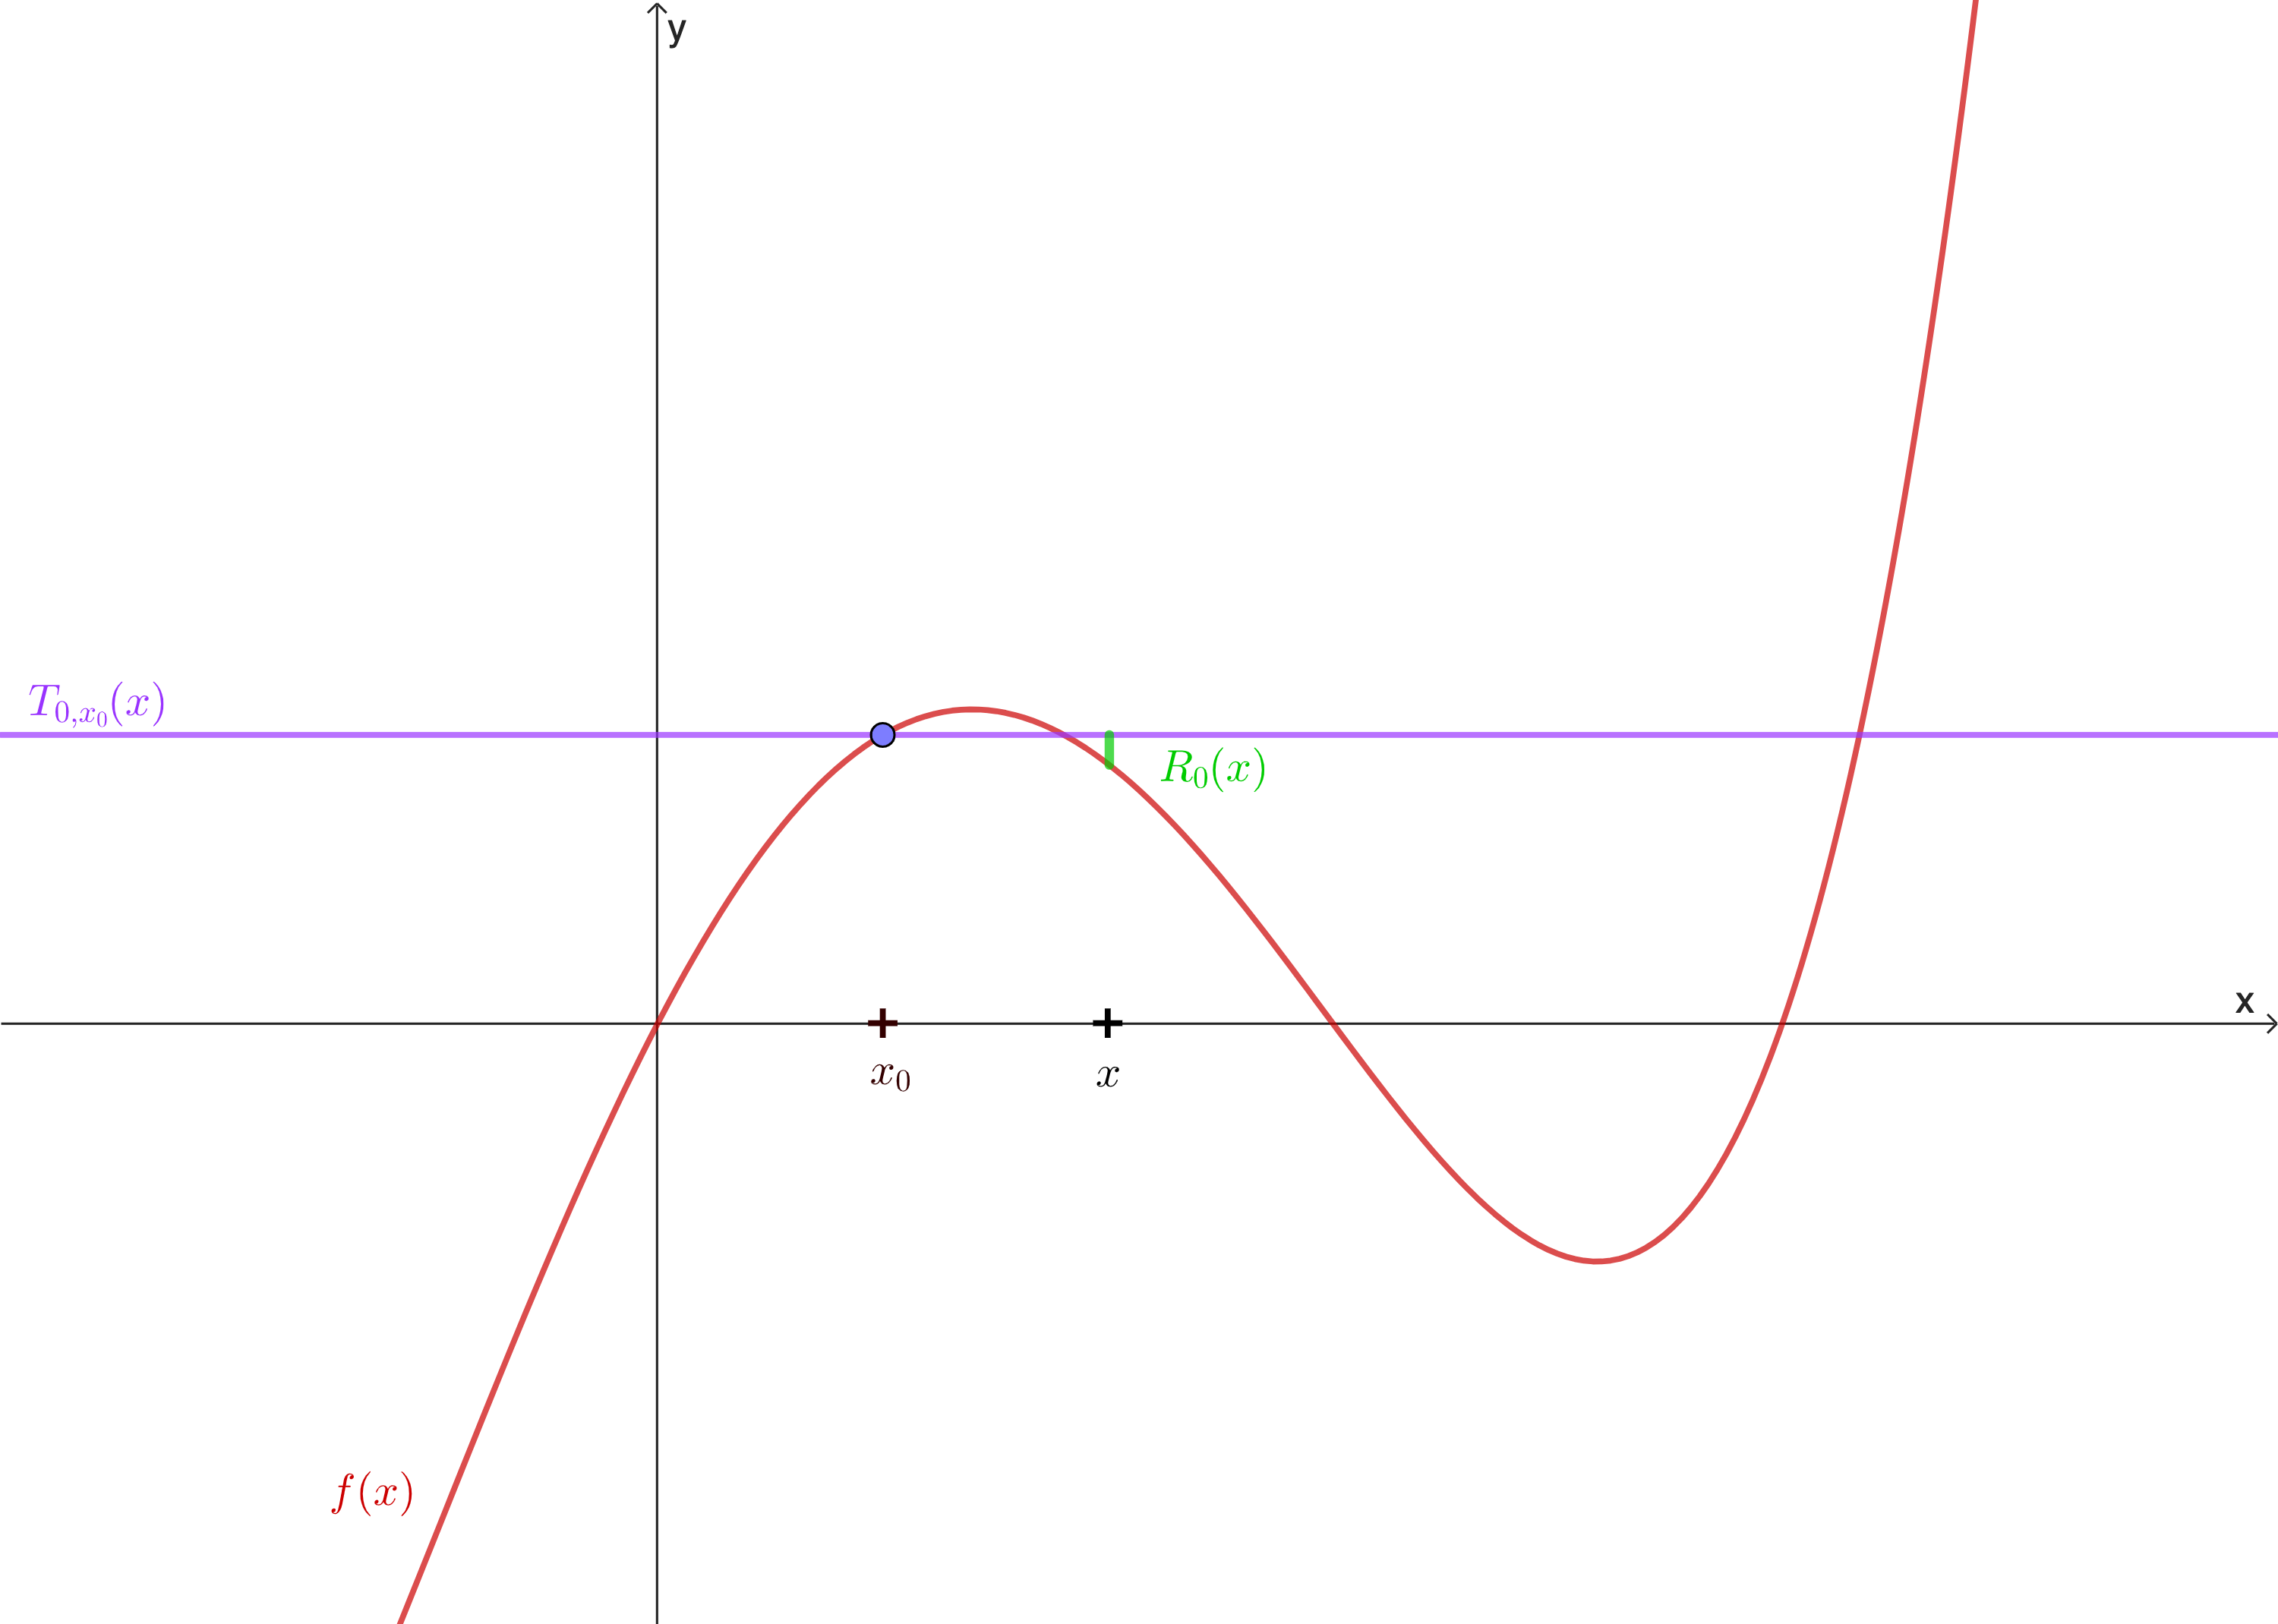
\includegraphics[width = 0.6 \textwidth]{media/BildRestglie0.png}
\end{center}

\begin{satz}
	{Restglied $R_0$ nach Lagrange}{}
	Sei $f$ stetig differenzierbar an der Stelle $x_0$. Für das 0. Restglied $R_0(x)$ der Taylorentwicklung gilt:
	$$R_0 (x)=  f'(c) \cdot (x-x_0)$$
	Für ein (nicht näher bekanntes) $c\in ]x_0, x[$.

\end{satz}
\begin{proof}

\end{proof}











\clearpage
% \textbf{Das Restglied $R_1(x)$}

% Sei \( f \) nun eine Funktion, die sich an der Stelle \( x_0 \) zweimal differenzieren lässt, und sei \( T_{1,x_0}(x) \) deren Taylorpolynom ersten Grades mit Entwicklungsstelle \( x_0 \), das heisst:
% \[ T_{1,x_0}(x) = f(x_0) + f'(x_0)(x - x_0) \]

% Das Restglied \( R_1(x) \) ist dann wieder die Differenz zwischen der Funktion \( f \) und der Taylorentwicklung \( T_{1,x_0}(x) \):
% \[ R_1(x) = f(x) - T_{1,x_0}(x) = f(x) - f(x_0) - f'(x_0)(x - x_0) \]
% \begin{center}
%     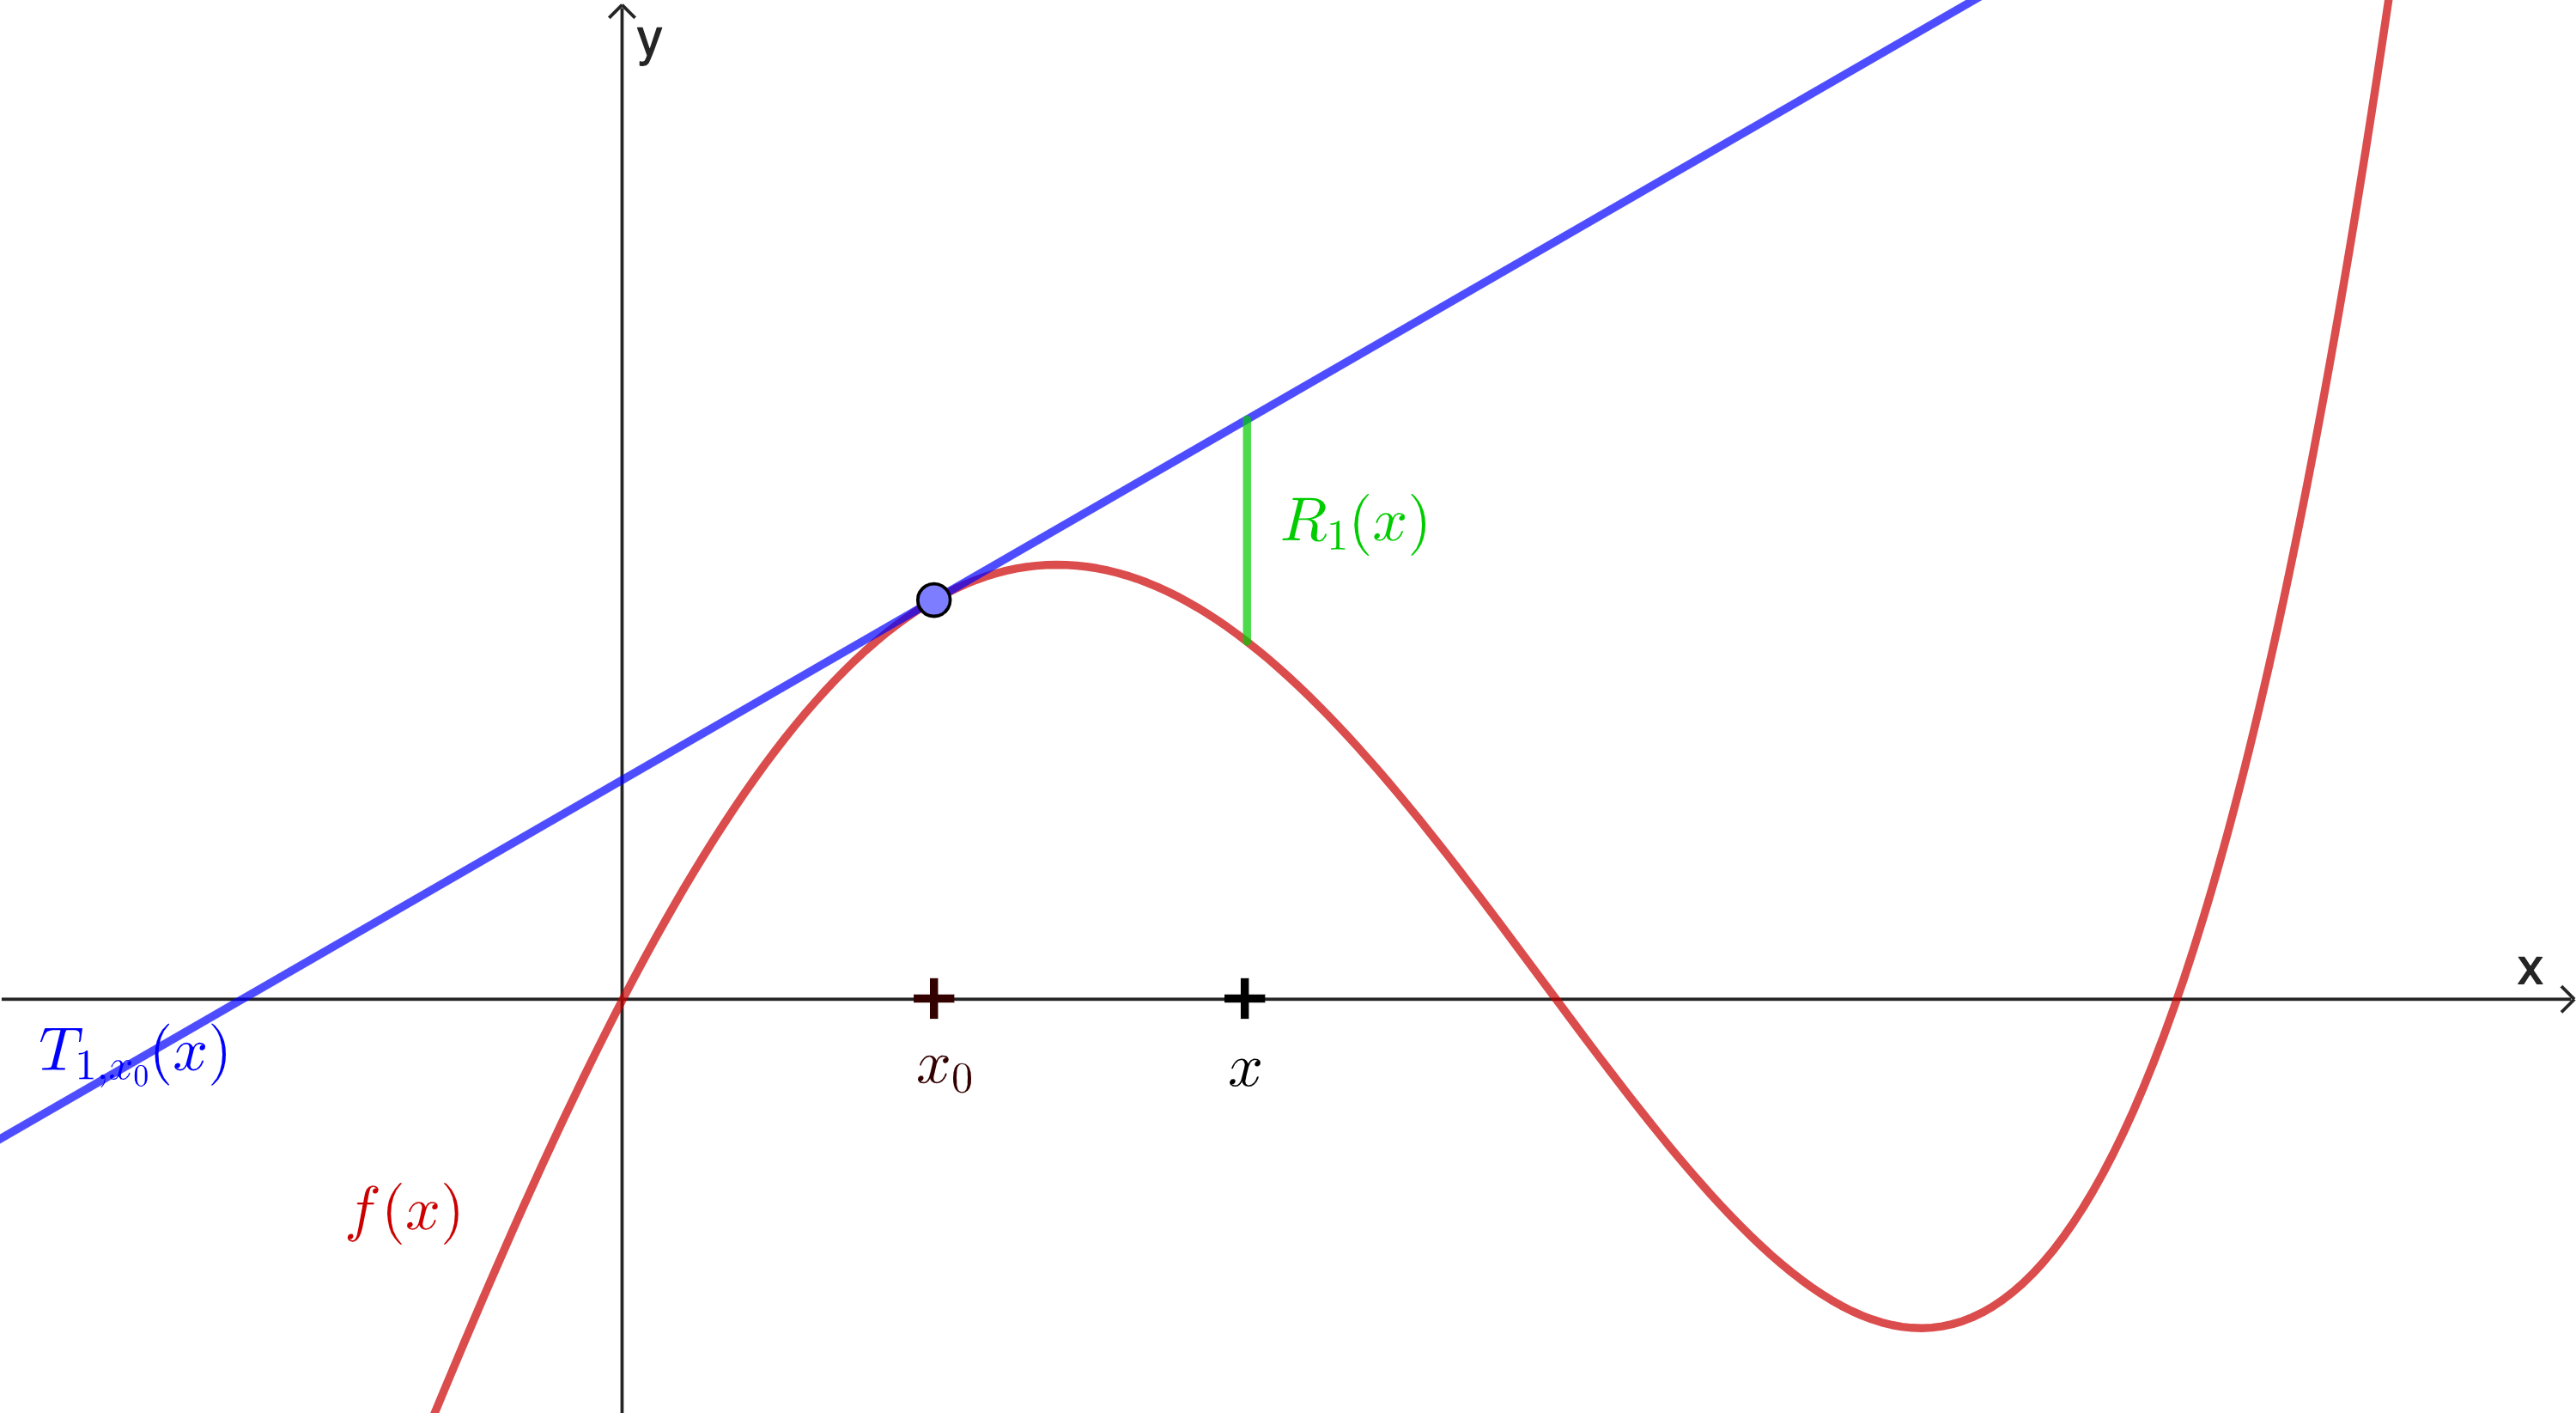
\includegraphics[width = 0.6 \textwidth]{media/BildRestglie1.png}
% \end{center}
% Nun wenden wir den 2. MWS auf die Funktionen $R_1 (x)$ und $g(x)=(x-x_0 )^2$ im Intervall $[x_0,x]$ an: (wird im Unterricht gemacht)
% \clearpage
% \begin{satz}
%     {Restglied $R_1$ nach Lagrange}{}
%     Sei $f$ zweimal stetig differenzierbar an der Stelle $x_0$. Für das 1. Restglied $$R_1 (x)=f(x)-T_{1,x_0 } (x)$$ gilt:
%     $$R_1 (x)= \qquad\qquad\qquad$$                                               

%     \vspace*{0.2cm}

% \end{satz}

% Mit dieser Formel für das Restglied kann man Abschätzen, welchen Fehler man macht, wenn man den Wert einer Funktion durch die konstante Approximation der Funktion annähert. 

% Versetzen Sie sich dazu in die Lage eines Ingenieurs in den Siebzigerjahre. Taschenrechner gibt es noch nicht. Um den Wert von $\sin(1^\circ)$ zu berechnen, verwendet er die Taylorapproximation 1. Grades. Der Fehler darf aber nicht grösser als $10^{-3}$ sein.  

% \begin{bsp}
%     {Fehler bei Approximation von $\sin(1^\circ)$ durch das Taylorpolynom 1. Grades (wird im Unterricht gemacht)}{} 

%     \vspace{13cm}
% %     Nutzen wir das Restglied von Lagrange einmal exemplarisch, um den Fehler abzuschätzen, den man macht, wenn man \(\sin(31^\circ)\) mithilfe der linearen Approximation der Sinusfunktion an der Stelle \(x_0 = 30^\circ\) annähert. Um besser ableiten zu können, müssen wir im Bogenmass rechnen: \(30^\circ \rightarrow \pi/6\), \(31^\circ \rightarrow 31\pi/180\), \(1^\circ \rightarrow \pi/180\).

% % Dann lautet das Taylorpolynom 1. Grades der Sinusfunktion an der Entwicklungsstelle \(x_0 = \pi/6\):
% % \[ T_{1,\pi/6}(x) = \sin(\pi/6) + \cos(\pi/6) \cdot (x-\pi/6) \]

% % Damit folgt für \(x = (31\pi)/180\):
% % \[ \sin(31^\circ) \approx T_{1,\pi/6}\left(\frac{31\pi}{180}\right) = \sin(\pi/6) + \cos(\pi/6) \cdot \left(\frac{31\pi}{180}-\pi/6\right) = \frac{1}{2} + \frac{\sqrt{3}}{2} \cdot \frac{\pi}{180} \approx 0.5151 \]

% % Den Fehler, den wir bei dieser Approximation machen, können wir nun mit dem Restglied nach Lagrange abschätzen:
% % \[ |R_1(31^\circ)| = |R_1(31\pi/180)| = \left|\frac{-\sin(c)}{2} \cdot \left(\frac{\pi}{180}\right)^2 \right| < \frac{1}{2} \cdot \left(\frac{\pi}{180}\right)^2 < 0.00015 \]

% \end{bsp}

Ähnlich wie die Formel für das 0. Restglied kann man auch jene für das $n$-te Restglied herleiten.
\begin{satz}
	{Restglied $R_n$ nach Lagrange}{}
	Sei \( f \) \((n+1)\)-mal stetig differenzierbar an der Stelle \( x_0 \). Für das \( n \)-te Restglied \( R_n(x) = f(x) - T_{n,x_0}(x) \) gilt:

	\[ R_n(x) = \frac{f^{(n+1)}(c)}{(n+1)!} \cdot (x - x_0)^{n+1} \]

	für ein (nicht näher bekanntes) \( c \in ]x, x_0[ \).

\end{satz}

In der Regel sorgt die Fakultät $(n+1)!$ im Nenner dafür, dass der Fehler für wachsendem $n$ immer kleiner wird. Man kann dann auch bestimmen, welcher Grad des Taylorpolynoms nötig ist, um eine bestimmte Genauigkeit zu garantieren.

\begin{bsp}
	{Approximation der Eulerschen Zahl $e$ mit vorgegebener Genauigkeit}{}
	Wir können wir Lagrange-Restglied verwenden, um die Zahl \(e\) mit einer Genauigkeit von \(10^{-6}\) zu berechnen. (Wird in der Klasse ergänzt)
	%    Dazu betrachten wir das Taylorpolynom \(n\)-ten Grades der Funktion \(e^x\) mit Entwicklungsstelle \(x_0 = 0\):
	% \[ T_n(x) = \sum_{k=0}^n \frac{x^k}{k!} \]
	% Für \(x = 1\) liefert uns \(T_n(1)\) eine Approximation für \(e\), wobei für den begangenen Fehler \(R_n(1) = e - T_n(1)\) nach Lagrange gilt: Es gibt ein \(c \in ]0, 1[\) mit
	% \[ R_n(1) = \frac{e^c}{(n+1)!} \cdot (1 - 0)^{n+1} = \frac{e^c}{(n+1)!} \]
	% Weil \(e^c < e^1 < 3\) ist, kann das Restglied grob abgeschätzt werden durch:
	% \[ R_n(1) < \frac{3}{(n+1)!} \]
	% Die angestrebte Genauigkeit von \(10^{-6}\) wird sicher erreicht, wenn
	% \[ |R_n(1)| < \frac{3}{(n+1)!} < 10^{-6} \implies 3 \cdot 10^6 < (n+1)! \implies n \geq 9 \]
	% Somit folgt, dass
	% \[ T_9(1) = \sum_{k=0}^9 \frac{1}{k!} = 1 + 1 + \frac{1}{2} + \frac{1}{6} + \frac{1}{24} + \frac{1}{120} + \frac{1}{720} + \frac{1}{5040} + \frac{1}{362880} =2.718281525573\ \]
	% sich um weniger als \(10^{-6}\) vom exakten Wert von $e$ unterscheidet.

	\vspace{13cm}

\end{bsp}
\clearpage
\begin{ueb}
	{}{}
	\begin{enumerate}
		\item 	Approximieren Sie den Wert von $f(x)$ durch das Taylorpolynom 1. Grades mit Entwicklungsstelle $x_0$. Schätzen Sie anschliessen den Fehler mit dem Lagrange-Restglied ab.
		      \begin{enumerate}
			      \item 	$f(x)=\ln(x), \, x_0=1, \,   x=1.01$
			      \item  	$f(x)=\frac{1}{\sqrt{x+1}}, \, x_0=0, \,   x=0.01$
			      \item  $f(x)=\sin(x), \, x_0=0,  \,  x= \frac{\pi}{180} \left(= 1^\circ\right)$
		      \end{enumerate}
		\item  	Bestimmen Sie das Taylorpolynom 3. Grades der Funktion $f(x)=\sin^2(x)=(\sin(x) )^2$ mit Entwicklungsstelle $x_0=0$ und zeigen Sie, dass dieses Polynom die Funktion $f$ im Intervall $\left[0,\frac{1}{2}\right]$ mit einer Genauigkeit von $\frac{1}{48}$ approximiert.

	\end{enumerate}
\end{ueb}
\clearpage
\emph{Lösungen:}
\begin{enumerate}
	\item  Approximationen
	      \begin{enumerate}
		      \item \( \ln(1.01) \approx 0.01, \,  |R_1(1.01)| < 0.00005 \)
		      \item \( f(0.01) \approx 0.995, \, |R_1(0.01)| < 3.75 \cdot 10^{-5} \)
		      \item  \( \sin\left(\frac{\pi}{180}\right) \approx \frac{\pi}{180} , \, \left|R_1\left(\frac{\pi}{180}\right)\right| < 0.00015 \)


	      \end{enumerate}

	\item Mit Kettenregel und Produktregel findet man: \( f'(0) = 0, f''(0) = 2, f'''(0) = 0 \).
	      Damit findet man \( T_3(x) = x^2 \).
	      Ausserdem ist \( |f^{(4)}(c)| = |8(1-2 \cos^2(c))| \leq 8 \implies \dots \implies |R_3(x)| \leq \frac{1}{48} \).


\end{enumerate}
\clearpage

\subsection{Konvergenz von Taylorreihen}

Mit der Formel für das $n$-te Restglied nach Lagrange können wir nun zeigen, dass die Taylorreihe der Sinusfunktion tatsächlich an jeder Stelle gegen $\sin(x)$ konvergiert. Dazu benötigen wir allerdings noch eine Zutat:
\begin{satz}
	{Fakultäten wachsen schneller als Exponentialfunktionen}{}
	\[\lim_{{n \to \infty}} \frac{|x|^n}{n!} = 0\] für jedes \(x \in \mathbb{R}\).

\end{satz}
\begin{proof}
	Die Folge \(a_n = \frac{|x|^n}{n!}\) kann rekursiv definiert werden als \(a_1 = x\), \(a_n = a_{n-1} \cdot \frac{|x|}{n}\). Wenn \(|x|\) sehr gross ist (z.B. \(|x| = 100\)), werden die ersten Glieder der Folge sehr schnell wachsen. Ab einem bestimmten Zeitpunkt wird \(n\) aber \(|x|\) überholen (z.B. ab dem 101. Glied). Danach werden die Folgenglieder immer kleiner. Sobald \(n > 2 \cdot |x|\) ist, werden die Folgenglieder jedes Mal mindestens halbiert. Damit konvergiert die Folge gegen Null.

\end{proof}
\begin{satz}
	{Konvergenz der Taylorentwicklung von $\sin(x)$}{}
	Die Taylorreihe \(T(x) = T_0(x) = \sum_{k=0}^{\infty} \frac{(-1)^k}{(2k+1)!} x^{2k+1}\) der Funktion \(f(x) = \sin(x)\) konvergiert für jedes \(x \in \mathbb{R}\) gegen \(f(x)\).

\end{satz}
\textit{Beweis:}

% \begin{proof}
%     \vspace{3cm}
% %     Für das \(n\)-te Restglied gibt es nach Lagrange ein \(c \in ]0, x[\):
% % \[ |R_n(x)| = \left| \frac{f^{(n+1)}(c)}{(n+1)!} \cdot x^{n+1} \right| =
% % \begin{cases}
% % \left| \frac{\cos(c)}{(n+1)!} \cdot x^{n+1} \right|, & \text{falls } n \text{ gerade} \\
% % \left| \frac{\sin(c)}{(n+1)!} \cdot x^{n+1} \right|, & \text{falls } n \text{ ungerade}
% % \end{cases} \leq \left| \frac{1}{(n+1)!} \cdot x^{n+1} \right| \]

% % Weil Fakultäten schneller wachsen als Exponentialfunktionen gilt nun:
% % \[ 0 \leq \lim_{{n \to \infty}} |R_n(x)| \leq \lim_{{n \to \infty}} \frac{x^{n+1}}{(n+1)!} = 0 \implies \lim_{{n \to \infty}} |R_n(x)| = 0 \]

% \end{proof}
\clearpage

\begin{ueb}
	{}{}
	\begin{enumerate}
		\item	Beweisen Sie, dass die Taylorreihe von $f(x)=e^x$ mit Entwicklungsstelle $x_0=0$ gegen $e^x$ konvergiert.

		\item Bei der Beschreibung von Hyperbeln spielen die Funktionen  $y= \frac{e^x - e^{-x}}{2}$ und $y= \frac{e^x + e^{-x}}{2}$ eine wichtige Rolle. Diese werden mit \emph{Hyperbelfunktionen} bezeichnet. Weil sie sich ausserdem in vielen Eigenschaften den trigonometrischen Funktionen ähneln, werden sie mit $\sinh(x) = \frac{e^x - e^{-x}}{2}$ (für \emph{sinus hyperbolicus}) und $\cosh(x)=\frac{e^x + e^{-x}}{2}$ (für \emph{cosinus hyperbolicus}) abgekürzt.
		      \begin{enumerate}
			      \item Zeigen Sie, dass für die Ableitungen der Hyperbelfunktionen gilt: \(\frac{d}{dx} \sinh(x) = \cosh(x)\) und \(\frac{d}{dx} \cosh(x) = \sinh(x)\). (Das ist eine erste Analogie zu den trigonometrischen Funktionen.)
			      \item Zeigen Sie, dass für die Hyperbelfunktionen die Gleichung \(\cosh^2(x) - \sinh^2(x) = 1\) gilt. (Das ist eine zweite Analogie zu den trigonometrischen Funktionen.)
			      \item         Bestimmen Sie die Taylorreihe der Funktion \(\sinh(x) = \frac{e^x - e^{-x}}{2}\) mit Entwicklungsstelle \(x_0 = 0\) und zeigen Sie, dass diese für alle \(x \in \mathbb{R}\) gegen \(\sinh(x)\) konvergiert.
		      \end{enumerate}


		\item Wie wir beobachtet haben, konvergiert die Taylorreihe der Funktion \(f(x) = \ln(x+1)\) in der Nähe der Entwicklungsstelle \(x_0 = 0\). Andererseits divergiert sie, wenn $x$ zu weit von $0$ entfernt ist. Diesem Phänomen soll in den folgenden Aufgaben nachgegangen werden.
		      \begin{enumerate}
			      \item Zeigen Sie, dass die Taylorreihe der Funktion \(f(x) = \ln(x+1)\) um $x_0 = 0$ für alle \(x\) im Bereich \(-\frac{1}{2} < x < \frac{1}{2}\) gegen \(f(x)\) konvergiert.
			      \item Was läuft an der Argumentation aus (a) schief, wenn man analog die Konvergenz für $x=2$ zeigen möchte?
		      \end{enumerate}


	\end{enumerate}
\end{ueb}
\clearpage
\emph{Lösungen:}
\begin{enumerate}

	\item Das Wesentliche: \( |R_n(x)| \leq \left|e^x \cdot \frac{x^{n+1}}{(n+1)!} \right| \rightarrow 0 \)



	\item
	      \begin{enumerate}
		      \item Folgt direkt mit der Kettenregel.
		      \item Lässt sich leicht aus der Definition und den binomischen Formeln herleiten.
		      \item Das Wesentliche: \( T(x) = \sum_{k=0}^n \frac{x^{2k+1}}{(2k+1)!} \), \( |R_n(x)| \leq \left|e^{|x|} \cdot \frac{x^{n+1}}{(n+1)!}\right| \rightarrow 0 \)
	      \end{enumerate}

	\item
	      \begin{enumerate}
		      \item Das ist etwas knifflig mit den Abschätzungen\dots

		            Das Wesentliche: \( |R_n(x)| \leq \frac{1}{n+1} \cdot \left(\frac{x}{c+1}\right)^{n+1} \leq \frac{1}{n+1} \cdot \left(\frac{\frac{1}{2}}{\frac{1}{2}}\right)^{n+1} \rightarrow 0\)
		      \item Für den Worst-Case $c=0$ erhält man die Abschätzung
		            $$|R_n(x)| \leq \frac{2^{n+1}}{n+1}$$
		            die für $n\to \infty$ nicht gegen Null strebt.
	      \end{enumerate}
\end{enumerate}


\begin{ueb}
	{Programmieraufgabe}{}
	Der folgende Python-Code berechnet eine Approximation für die Zahl $\sin(\pi/4)$ mit der Taylorentwicklung 19. Grades des Sinusfunktion.
	$$ \sin(x) \approx \sum_{i=0}^{9} \frac{(-1)^i}{(2i+1)!} \cdot x^{2i+1}$$
	\lstinputlisting{programme/sinus_approx.py}
	\begin{enumerate}
		\item Kopieren Sie den Code und lassen Sie ihn laufen.
		\item Berechnen Sie mit dem Programm eine Approximation für Winkel, die etwas weiter von $0$ entfernt sind und beobachten Sie, wie der Fehler zunimmt.
		\item Schreiben Sie ähnliche Programme zur Approximation anderer Funktionen, z.B. $\cos(x)$, $e^x$, $\ln(x)$, \dots
	\end{enumerate}
\end{ueb}

% \begin{ueb}
% 	{Programmieraufgabe für Experten}{}
% 	Schreiben Sie ein Python-Programm, dass die Taylorapproximation einer beliebigen Funktion an einer beliebigen Stelle bis zu einem gewünschten Grad berechnet.

% 	Einige Meilenteine:
% 	\begin{enumerate}
% 		\item Schreiben Sie ein Python-Funktion, die als Eingabe eine Funktion $f$ und eine Stelle $x_0$ erhält und eine Näherung für den Wert der Ableitung $f'(x_0)$ zurückgibt. Verwenden Sie dazu den Differenzenquotienten $\frac{f(x_0 + h) - f(x_0)}{h}$ mit einem kleinen $h$ (z.B. $h=10^{-5}$).
% 		\item Schreiben Sie eine Python-Funktion, die als Eingabe eine Funktion $f$, die Entwicklungsstelle $x_0$ und eine Stelle $x$ erhält und den Wert der Taylorapproximation 1. Grades mit Entwicklungsstelle $x_0$ von $f$ an der Stelle $x$ zurückgibt.
% 		\item Schreiben Sie eine Funktion , die als Eingabe eine Funktion $f$ erhält und die Ableitungsfunktion $f'$ zurückgibt. (Der Rückgabewert kann auch eine Python-Funktion sein!)
% 		\item Schreiben Sie ein Programm, das als Eingabe eine Funktion $f$ und eine Zahl $n$ erhält und die $n$-te Ableitung $f^{(n)}$ zurückgibt.
% 		\item Schreiben Sie nun eine Funktion, die als Eingabe eine Funktion $f$, die Entwicklungsstelle $x_0$, eine Stelle $x$ und einen Grad $n$ erhält und den Wert der Taylorapproximation $n$-ten Grades mit Entwicklungsstelle $x_0$ von $f$ an der Stelle $x$ zurückgibt.

% 	\end{enumerate}
% \end{ueb}
